\documentclass[tikz,border=8pt]{standalone}
% Shared look for every TikZ diagram. Load with \input{../../tools/tikz-style.tex}
\usepackage[sfdefault]{roboto}
\usetikzlibrary{arrows.meta, positioning, shapes.geometric, calc, fit, backgrounds}
\definecolor{cblue}{HTML}{4C78A8}
\definecolor{corange}{HTML}{F58518}
\definecolor{cgreen}{HTML}{54A24B}
\definecolor{cred}{HTML}{E45756}
\definecolor{cpurple}{HTML}{B279A2}
\definecolor{cgrey}{HTML}{6B6B6B}
\tikzset{
  every picture/.style={font=\sffamily, line width=1.2pt},
  box/.style={draw=#1, fill=#1!12, rounded corners=4pt, align=center, inner sep=7pt, minimum height=1.1cm},
  box/.default=cgrey,
  arrow/.style={-{Stealth[length=3mm]}, draw=cgrey, line width=1.4pt},
  title/.style={font=\sffamily\bfseries\Large},
  note/.style={font=\sffamily\small, text=cgrey, align=center},
}
\AtBeginDocument{\hyphenpenalty=10000 \exhyphenpenalty=10000}

% Bilinear interpolation at the end of the robot's first move (dp_anim.py): from (2, 1), 0.5 m at 67.5 degrees, to
% p = (2.191, 1.462) m. The four cell centres around p: (1.75, 1.25), (2.25, 1.25) = S's centre, (1.75, 1.75) and
% (2.25, 1.75), with their cost-to-go after dynamic programming with interpolation, 16 moves (gridplan.dp_interp):
% 3.557, 3.338, 3.122 and 2.862 m. p is 0.8827 of the way across and 0.4239 of the way up. Each centre's weight is
% the area of the rectangle on the far side of p from it: 0.0676, 0.5085, 0.0497, 0.3742. Blend: 3.164 m.
% Scale: 1 m = 16 cm.
\begin{document}
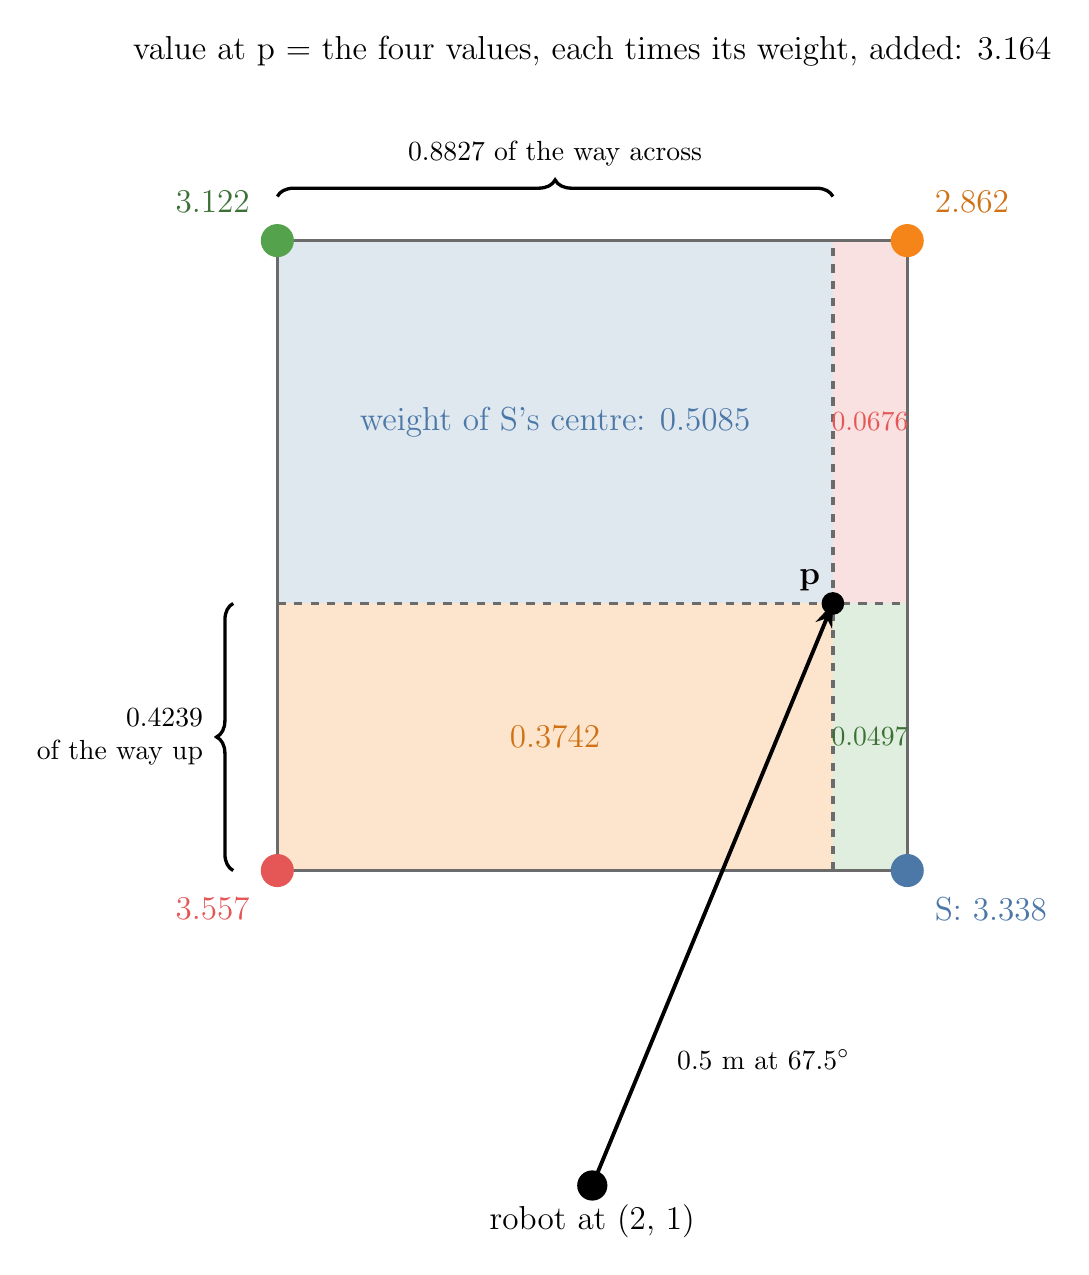
\begin{tikzpicture}[x=16cm, y=16cm, every node/.append style={font=\large},
  ctr/.style={circle, fill=#1, minimum size=0.42cm, inner sep=0pt}]
  \def\px{2.191}\def\py{1.462}
  % the four rectangles, each in the colour of the centre whose weight it is (the one diagonally opposite)
  \fill[cred!18]    (\px,\py) rectangle (2.25,1.75);   % weight of bottom-left
  \fill[cblue!18]   (1.75,\py) rectangle (\px,1.75);   % weight of bottom-right (S)
  \fill[cgreen!18]  (\px,1.25) rectangle (2.25,\py);   % weight of top-left
  \fill[corange!22] (1.75,1.25) rectangle (\px,\py);   % weight of top-right
  \draw[cgrey] (1.75,1.25) rectangle (2.25,1.75);
  \draw[cgrey, dashed] (\px,1.25) -- (\px,1.75);
  \draw[cgrey, dashed] (1.75,\py) -- (2.25,\py);
  % weights written in the rectangles
  \node[text=cred, font=\normalsize] at ({(\px+2.25)/2},{(\py+1.75)/2}) {0.0676};
  \node[text=cblue] at ({(1.75+\px)/2},{(\py+1.75)/2}) {weight of S's centre: 0.5085};
  \node[text=cgreen!70!black, font=\normalsize] at ({(\px+2.25)/2},{(1.25+\py)/2}) {0.0497};
  \node[text=corange!85!black] at ({(1.75+\px)/2},{(1.25+\py)/2}) {0.3742};
  % centres and their values
  \node[ctr=cred]    (a) at (1.75,1.25) {};  \node[below left=2pt of a, text=cred] {3.557};
  \node[ctr=cblue]   (b) at (2.25,1.25) {};  \node[below right=2pt of b, text=cblue] {S: 3.338};
  \node[ctr=cgreen]  (c) at (1.75,1.75) {};  \node[above left=2pt of c, text=cgreen!70!black] {3.122};
  \node[ctr=corange] (d) at (2.25,1.75) {};  \node[above right=2pt of d, text=corange!85!black] {2.862};
  % the robot's move
  \fill[black] (2,1) circle (0.012);
  \node[below=3pt, font=\large] at (2,1) {robot at (2, 1)};
  \draw[arrow, draw=black] (2,1) -- (\px,\py);
  \node[right=4pt, font=\normalsize, align=left] at (2.05,1.1) {0.5 m at 67.5$^\circ$};
  \fill[black] (\px,\py) circle (0.009);
  \node[above left=1pt, font=\large\bfseries] at (\px,\py) {p};
  % fractions
  \draw[decorate, decoration={brace, amplitude=6pt}] (1.75,1.785) -- node[above=7pt, font=\normalsize] {0.8827 of the way across} (\px,1.785);
  \draw[decorate, decoration={brace, amplitude=6pt}] (1.715,1.25) -- node[left=7pt, font=\normalsize, align=right] {0.4239\\of the way up} (1.715,\py);
  \node[font=\large, align=center] at (2.0,1.9) {value at p $=$ the four values, each times its weight, added: 3.164};
\end{tikzpicture}
\end{document}
